\chapter{Introduction}


In questo capitolo ci occuperemo di analizzare e comprendere delle vulnerabilità
del protocollo DDS standard OMG (Object Managment Group). In particolare
verrà analizzato il vettore d'attacco, il protocollo utilizzato, il bersaglio
dell'attacco e infine verrà proposta una soluzione applicabile per
mitigare possibili attacchi non autorizzati. Successivamente grazie all'aiuto 
di un software riusciremo a capire come queste vulnerabilità possono 
influire sul funziomanto degli --host-- collegati alla rete DDS. In molti casi
l'attaccante ha a disposizione un dispositivo all'interno della rete sotto
il suo controllo.


\section{Attacchi di tipo DDoS}
Questo attacco consiste nel sovraccaricare un dispositivo collegato alla rete DDS
in modo tale da renderlo inutilizzabile. Infatti dato che i dispositivi collegati
sono di -- tipo I O T -- la potenza di calcolo nella maggior parte dei casi sarà
molto ridotta. Inoltre in molti casi ci possiamo ritrovare ad utilizzare dispositivi
che non possono permettersi --delay-- nell'analisi di certi dati, specialmente in
ambiti dove bisogna avere una risposta sempre rapida e disponibile, come ad esempio
nel campo della medicina e nel campo militare.


\subsection{DDoS blocco ricezione da parte del data-reader Foglio 2}

%\subsubsection{Prologo}
Citazioni da foglio 2 a gogo
Il vettore di attacco si trova nell'implementazione del DDS chiamata DDSI-RTPS che
si occupa di scambiare messaggi tra i data-reader (coloro che si iscrivono ai vari
ai vari topic) e i data-subscribers (di solito sono sensori che mandano dati). Per
comunicare questi dispositivi utilizzano il protocollo RTPS. 
Questo protocollo utilizza il messaggio HEARTBEAT che viene mandato da un data-writer 
a un data-reader per specificare il sequence number nel data-writer.
All'interno del messaggio HEARTBEAT troviamo il sequence number che serve al 
data-reader per sincronizzarsi con il data-writer durante la ricezione dei messaggi. 
Infatti il data-reader quando riceve il sequence number all'interno di un HEARTBEAT
può identificare se ci sono dei pacchetti mancanti e segnalarli al
data-writer.

Un data-writer inoltre può richiedere un messaggio ACKNACK da un data-reader se 
nel messaggio HEARTBEAT inviato dal data-writer viene specificata la flag FINAL.
In casi in cui bisogna essere certi che il data-reader riceve tutti i dati del
data-writer, quest'ultimo manda un HEARTBEAT con la flag FINAL impostata, al
data-reader che successivamente deve rispondere necessariamente con un messaggio
ACKNACK per confermare la ricezione nel messaggio HEARTBEAT.
I controlli HEARTBEAT effettuati dal data-reader,
infatti non sono sufficienti a coprire questo tipo di attacco
dato che quest'ultimo:
\begin{itemize}
    \item esegue un check per verificare che non vi siano numeri negativi
    \item controlla che l'ultimo sequence number arrivato non ha un valore più alto 
    del sequence number ricevuto in precedenza 
\end{itemize}
\subsubsection{Dettagli attacco AFTER}
Per sfruttare questa vulnerabilità l'attaccante deve utilizzare qualche strumento
per sniffare la comunicazione tra data-reader e data-writer e intercettare un
messaggio di tipo HEARTBEAT. Successivamente l'attaccante modifica il valore del
sequence number del messaggio HEARTBEAT. Il messaggio poi viene mandato verso il
data-writer così facendolo rimanere in attesa di un messaggio HEARTBEAT con Un
sequence number superiore a quello appena ricevuto. Facendo così il data-reader
non legge più i messaggi mandati dal data-writer e bloccando così l'esecuzione
del data-reader finchè il sequence number non 
sarà superiore a quello ricevuto dall'attaccante.

\subsubsection{Conclusioni AFTER}
Di solito questi tipo di attaco sono difficili da identificare.

\subsection{DDoS sfruttando estensione DDS security}
In questo attacco dobbiamo considerare il modulo del DDS chiamato DDS security
versione 1.1.(fonti ora da foglio 6) Questo modulo si occupa di stabilire una
connessione sicura tra i vari dispositivi della rete. Infatti verranno utilizzate
delle api da parte dei partecipanti per effettuare le varie azioni, come
ad esempio iscriversi ad un topic e pubblicare un messaggio del topic.
(foglio 3 pag 718)Per effettuare l'autenticazione un partecipante deve prima
risolvere una challenge criptografica richiesta dal sistema di autenticazione
della rete. Effettuato poi questo calcolo criptografico il risultato viene
controllato dal sistema di autenticazione, controllando che se il risultato
inviato corrisponde all'hash della challenge criptografica.

\subsubsection{Dettagli attacco AFTER foglio 3}
L'attacco DDoS si svolge proprio durante la fase di autenticazione del protocollo
DDS security 1.1, in particolare quando un nuovo dispositivo legittimo si vuole 
collegare alla rete e comincia a mandare una richiesta di autenticazione
all'ente di controllo. La richiesta del partecipante poi viene intercettata 
dall'attaccante che modifica i valori all'interno del pacchetto delle 
challenge criptografica. Modicando ogni volta questi valori, l'attaccante
comincia a mandare tante richeieste criptografiche alla sua vittima.
Il partecipante comincierà a calcolare queste challenge per effettuare 
l'autenticazione investendo tutte le risorse necessarie.
Dato che molto probabilmente chi riceve questo attacco è un dispositivo IOT 
che non dispone di una potenza di calcolo molto elevata e si ritroverà
occupato per tutto il tempo necessario per risolvere le challenge criptografiche
ricevute dall'attaccante, bloccando così il suo funziomanto.

\subsubsection{Conclusioni AFTER foglio 3}
Una raccomandazione per mitigare questo attacco può essere quello di cambiare delle
policy QoS in modo tale da impostare un tempo limite massimo per effettuare
l'autenticazione. Impostando un limite simile queste policy possono prevenire
che i partecipanti si ritrovino sopraffatti dalle troppe richieste di 
autenticazione. Un allarme potrebbe essere anche utile per identificare possibili
tentativi DDoS di questo tipo così allertando un amministratore. (parlare di proverif)

\section{Attacchi di tipo Discovery}
Dal foglio 2
Prendere informazioni DDS senza effettuare veri e propri
attacchi di tipo attivo può essere molto utile per un attaccante che prova
a penetrare una rete DDS. In molti casi tutto quello che deve fare l'attaccante
è osservare i messaggi che vengono scambiati all'interno del network.
Successivamente quando si ottengono informazioni a sufficienza sarà più
facile per l'attaccante trovare un vettore di attacco.

\subsection{Enumeration sniff foglio 2 e foglio 5}
Prendendo in considerazione il protocollo DDSI-RTPS, possiamo notare che di
default quest'ultimo è molto "verbouse", cioè scambia molte informazioni in
chiaro durante le comunicazioni tra i vari dispositivi. In particolare
il modulo discovery del protocollo RTPS che a sua volta si suddivide in
altri 2 protocolli fondamentali che sono necessari:(foglio 5 pag 123)
\begin{itemize}
    \item Simple Partipant Discovery Protocol (SPDP)
    \item Simple Endpoint Discovery Protocol (SEDP)
\end{itemize}
Per questo attacco ci focalizzeremo in particolare nel SPDP che serve a
individuare la presenza dei partecipanti alla rete. In particolar modo
il funzionamento si basa su un messaggio di tipo multicast e unicast che viene
mandato a tutti i dispositivi della rete per informare chi è presente attualmente.
(foglio 5 pag 125)

\subsubsection{Dettagli attacco AFTER}
Utilizzando un qualche software in grado di "sniffare" i vari pacchetti della
rete, come un semplice script python è stato possibile analizzare il loro
contenuto. I pacchetti analizzati sono quelli di tipo multicast RTPS SPDP
All'interno di un pacchetto di questo tipo possiamo trovare: (nel foglio 2 
non viene specificato bene di quale pacchetto si parla, ma guardando la documentazione
da pag 125 del foglio 5, stiamo analizzando il pacchetto SPDPdiscoveredParticipandData)
(da scrivere in corsivo) l'indirizzo ip dell'host, il prefisso GUID dell'RTPS,
la versione dell RTPS, L'ID del venditore, informazioni riguardanti la sincronizzazione
e infine il contenuto dei submessages.


\subsubsection{Conclusioni AFTER}
Di solito questi tipo di attaco sono difficili da identificare e possono essere
effettuati anche non avendo un dispositivo autenticato all'interno della rete.

\section{Attacchi sfruttando le policy QoS foglio 1}

% \begin{figure}[H]
%     \centering
%     \includesvg[width=15cm,keepaspectratio]{img/Policy QoS DDS.drawio.svg}
%     \caption{Illustrazione policy QoS del DDS}\label{Mappa QoS svg}
% \end{figure}


\begin{figure}[H]
	\centering
    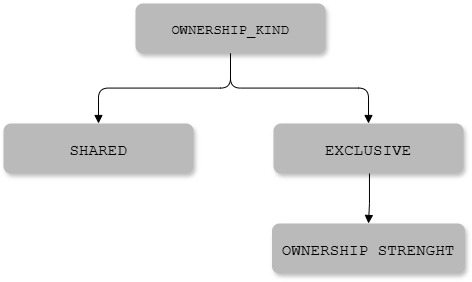
\includegraphics[width=10cm, keepaspectratio]{img/Policy QoS DDS_2.jpg}
	\caption{Illustrazione policy QoS del DDS}\label{Mappa QoS}
\end{figure}
% AFTER si potrebbe fare nei capitoli introduttivi una mappa che racchiuda
% i tipi di variabili che usano i QoS (int, double,.. etc) per i capitoli
% che spiegano meglio i concetti introduttivi

Queste tipologie di attacco sono possibili solo se certe policy QoS vengono
modificate durante l'esecuzione della rete, specialmente il parametro 
OWNERSHIP-KIND che gestisce quanti DataWriter possono scrivere per un
determinato Topic. Questo parametro può essere impostato in due modi diversi:
\begin{itemize}
    \item SHARED: in questo modo più di un DataWriter possono aggiornare le
    informazioni di un topic. Inoltre un DataReader si può iscrivere a
    qualsiasi scrittore dello stesso topic.
    \item EXCLUSIVE: solo un DataWriter può aggiornare le informazioni di un
    topic. Il DataWriter che ha il permesso di scrittura per il topic è quello
    che dispone di un OWNERSHIP-strength con valore più alto.
\end{itemize}

% https://www.omgwiki.org/ddsf/doku.php?id=ddsf:public:guidebook:06_append:02_quality_of_service:ownership
% https://www.omgwiki.org/ddsf/doku.php?id=ddsf:public:guidebook:06_append:02_quality_of_service:ownership_strength

\subsection{Foglio 4-B Modifica maligna di ownership strength}
In una rete dove si utilizza un OWNERSHIP-kind di tipo EXCLUSIVE è possibile
utilizzare l'OWNERSHIP-strength a favore
dell'attaccante. Infatti è possibile far ricevere informazioni a un DataWriter
in maniera errata, dato che quest'ultimo non riceverà più informazioni da
una fonte affidabile.

\subsubsection{Foglio 4-B Dettagli attacco}
L'attaccante, con un DataWriter in suo possesso all'interno di una rete DDS,
può sfruttare il fatto che il topic preso di mira può essere aggiornato
solo dal DataWriter con l'OWNERSHIP-strength più alta. 
Per effettuare questo attacco tutto quello che serve è sapere il topic che
si vuole modificare, le policy QoS in uso e il valore dell'ownership-strength.
L'ultimo passo è quello di impostare il topic scelto nel DataWriter
dell'attaccante con OWNERSHIP-strength superiore a quella utilizzata dal
DataWriter originario che aggiorna il topic.
Ora i DataReader che sono iscritti al topic bersaglio
ricevono le informazioni dal DataWriter dell'attaccante.

\subsubsection{Foglio 4-B Conclusioni}
L'OWNERSHIP-kind di tipo EXCLUSIVE è utilizzata in contensti dove le
informazioni ricevute dal DataReader devono essere accurate dato che un singolo
scrittore (in molti casi si tratta di un sensore) può mandare nuovi aggiornamenti
del topic. Se l'attaccante, dovesse riesce a modificare i valori del topic con
questo attacco, può causare in certi casi molti danni a seconda della rete DDS, 
specialmente se il DataWriter dell'attaccante riesce a mandare degli aggiornamenti
del topic senza che venga scoperto.



\subsubsection{Questa è una sottosottosezione}
La teoria dell'attacco ci dice che se 

% Definizione di un colore personalizzato
\definecolor{customgray}{rgb}{0.70, 0.70, 0.70} % Grigio chiaro

% Regolazione dello spessore delle linee
\setlength{\arrayrulewidth}{1.0pt} % Spessore linee generali
% \renewcommand{\arraystretch}{1.2} % Altezza righe


\begin{table}[H]
    \centering
    \rowcolors{2}{black!5}{white}
    \resizebox{\linewidth}{!}{%
        \begin{tabular}{|c|c|c|c|c|c|}
            \hline
            \rowcolor{customgray}
            \multicolumn{1}{|>{\columncolor{customgray}}c|}{\tabularCenterstack{c}{\textbf{Tipo di}\\ \textbf{attacco}}} &
            \multicolumn{1}{>{\columncolor{customgray}}c|}{\tabularCenterstack{c}{\textbf{Vettore} \\ \textbf{attacco}}} &
            \multicolumn{1}{>{\columncolor{customgray}}c|}{\tabularCenterstack{c}{\textbf{Protoc.}/ \\ \textbf{Estens.}}} &
            \multicolumn{1}{>{\columncolor{customgray}}c|}{\tabularCenterstack{c}{\textbf{Bersaglio} \\ \textbf{nella rete}}} &
            \multicolumn{1}{>{\columncolor{customgray}}c|}{\tabularCenterstack{c}{\textbf{Software}}} &
            \multicolumn{1}{>{\columncolor{customgray}}c|}{\tabularCenterstack{c}{\textbf{Soluzione}}} \\
            \hline
            \tabularCenterstack{l}{Discovery \\ devices[2]} &
            \tabularCenterstack{c}{Verbose nature \\ of RTPS} &
            \tabularCenterstack{c}{DDSI-RTPS} &
            \tabularCenterstack{c}{Tutti i par-\\tecipanti} &
            \tabularCenterstack{c}{Sniffer \\ python} &
            \tabularCenterstack{c}{-} \\
            \specialrule{0.3pt}{0pt}{0pt} % Linea più spessa dopo l'intestazione
            \tabularCenterstack{l}{DDos[2]} &
            \tabularCenterstack{c}{Heartbeat \\ sequence number} &
            \tabularCenterstack{c}{DDSI-RTPS} &
            \tabularCenterstack{c}{Data-reader} &
            \tabularCenterstack{c}{Sniffer \\ python} &
            \tabularCenterstack{c}{-} \\
            \specialrule{0.3pt}{0pt}{0pt} % Linea più spessa dopo l'intestazione
            \tabularCenterstack{l}{DDoS[3]} &
            \tabularCenterstack{c}{Authentication \\ challenge} &
            \tabularCenterstack{c}{DDS security 1.1 \\ Discovery protoc.} &
            \tabularCenterstack{c}{Tutti i par-\\tecipanti} &
            \tabularCenterstack{c}{Proverif} &
            \tabularCenterstack{c}{Scandenza richieste \\ di autenticazione} \\
            \specialrule{0.3pt}{0pt}{0pt} % Linea più spessa dopo l'intestazione
            
            % Aggiungere altre linee

            \hline
        \end{tabular}
        }
        \caption{La versione DDS in tutti i casi è la 1.4}
    \end{table}




